\documentclass[12pt,a4paper,UTF8]{article}
\usepackage{ctex} % Chinese support
\usepackage{graphicx} % Insert images
\usepackage{listings} % Print source code
\usepackage{color} % Color support
\usepackage{booktabs} % Professional table support
\usepackage{pdflscape} % Landscape pages support in PDF
\usepackage{hyperref} % Hypertext links support for cross-referencing

% Customize hyperref format (it's set to no special format here)
\hypersetup{hidelinks}

% Declare directories to search for graphics files for graphicx
\graphicspath{{figures/}{logo/}}

% Define source code style for listings
\lstdefinestyle{c}{
  language=C,
  basicstyle=\ttfamily\footnotesize,
  keywordstyle=\bfseries\color[rgb]{0, 0, 1},
  identifierstyle=\color[rgb]{0.2, 0.2, 0},
  stringstyle=\color[rgb]{0.6, 0.1, 0.1},
  commentstyle=\itshape\color[rgb]{0.05, 0.5, 0.05},
  backgroundcolor=\color[gray]{0.95},
  numbers=left,
  numbersep=5pt,
  numberstyle=\color[gray]{0.6},
  breaklines=true
}

% Define new command for title page
\newcommand{\reporttitle}[2]{
  \LARGE\textsf{#1}\quad\underline{\makebox[12em]{#2}}
}
\newcommand{\reportinfo}[2]{
  \large\makebox[4em]{\textsf{#1}}\quad\underline{\makebox[18em]{#2}}
}

% The document begins here
\begin{document}
\begin{titlepage}
  \centering
  \vspace*{\fill}
  
\includegraphics[height=144pt]{nju-logo}\\[48pt]
  {\huge\textsf{课\ 程\ 实\ 验\ 报\ 告}}\\[48pt]
  \reporttitle{实验名称}{文件系统}\\[72pt]

  \reportinfo{课程名称}{操作系统}\\[8pt]
  \reportinfo{院\hspace{\fill}系}{计算机科学与技术系}\\[8pt]
  \reportinfo{学\hspace{\fill}号}{191220129}\\[8pt]
  \reportinfo{姓\hspace{\fill}名}{邢尚禹}\\[8pt]
  \reportinfo{邮\hspace{\fill}箱}{191220129@smail.nju.edu.cn}\\[8pt]
  \reportinfo{实验日期}{2021年6月}\\
  \vspace*{\fill}
\end{titlepage}

\tableofcontents
\newpage
\section{实验进度}
已完成所有内容。

\section{实验思路和过程}
本次实验主要实现几个系统调用。
\subsection{open}
syscallOpen函数要对pcb和全局的文件描述符做一些修改,注意要充分考虑各种情况,如文件是否存在,文件是常规文件,设备文件还是目录,flag是否匹配等。
其执行流程大致如下。
\begin{itemize}
	\item 如果文件存在:
	\subitem 检查文件类型和打开文件的flag是否匹配;
	\subitem 检查文件是否已经被打开,此处不允许同一个文件被打开两次;
	\subitem 判断文件类型,如果是设备文件,直接返回文件id;如果是普通文件,修改pcb和全局文件描述符。
	\lstinputlisting[style=c]{open_exist.c}
	\item 如果文件不存在:
	\subitem 检查flag是否有create权限;
	\subitem 根据是普通文件还是目录做inode分配,写入磁盘;
	\subitem 建立新的文件描述符。
	\lstinputlisting[style=c]{open_create.c}
\end{itemize}
在实现中,要求出一个文件的父目录,可以直接从后到前查找符号'/',前面的字符串就是父路径,复制到一个新的缓冲区即可。框架代码提供了stringChrR和stringLen函数,用起来很方便。

\subsection{write}
syscallWriteFile需要把指定的内容从缓冲区写入磁盘,注意每次需要写一个block,故要设置两个变量,一个指示当前的字节数,一个指示当前的block位置。如果写入后的大小超出了inode限定的范围,则需要调用allocBlock分配一个新的block。如果allocBlock失败,需要立刻将已经写入的部分更新到文件描述符里。最后,调用diskWrite写入磁盘。
\lstinputlisting[style=c]{write.c}

\subsection{read}
syscallReadFile的实现相对简单,采用与write相同的两个变量指示位置,直接调用readBlock即可。
\lstinputlisting[style=c]{read.c}

\subsection{seek}
根据三种不同的基准(negin, current, end),直接修改全局文件描述符的偏移量。
\lstinputlisting[style=c]{seek.c}

\subsection{close}
先检查文件是否已被打开和是否是普通文件,如果是,直接将对应的描述符清零即可。
\lstinputlisting[style=c]{close.c}

\subsection{remove}
remove的关键操作就是freeInode,不过需要注意常规文件和目录文件的区别以及不能删除设备文件。另外,对于目录文件,如果最后一个字符是'/',要单独处理。获取父目录的方法与write相同。
\lstinputlisting[style=c]{remove.c}

\section{实验结果}
所有的系统调用都可以正确运行:
\begin{figure}[htbp]
	\centering
	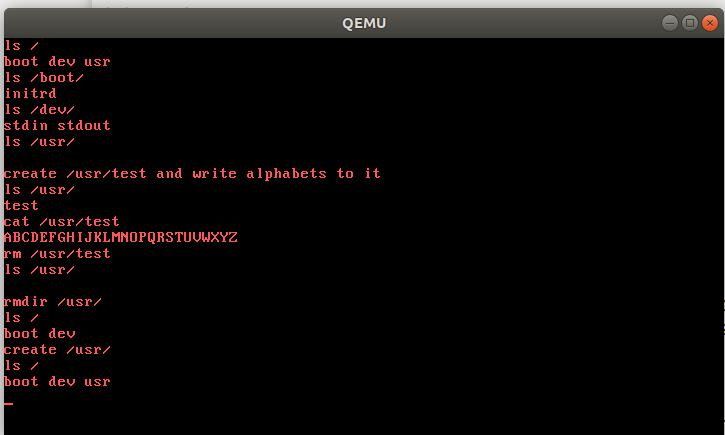
\includegraphics[width=\textwidth]{result}
	\caption{运行结果}
\end{figure}

\section{问题与思考}
\begin{enumerate}
	\item 20.04版本完全无法正常编译运行本次实验,即使代码正确,也会在第一个ls调用处卡住,尝试调试也没能发现问题。由于之前也出现过类似的问题(但通过修改bootloader和kvm的加载过程以及在Makefile中加编译参数可以解决),我就借用了同学的18.04编译,发现可以正常运行。暂时没有找到相关的解决方案。
	\item 在框架代码中有很多工具函数,如sreingLen, stringChrR等,使用很方便;也有关键性的函数接口,如freeInode等。但是,这些函数没有具体的说明(参数的字符串格式等)。一开始我错误地调用了这些函数,产生了一些bug,还很难找到,耗费了很多时间。
\end{enumerate}

\section{建议}
\begin{enumerate}
	\item 建议将官方的实验环境升级到20.04LTS版本。因为自己安装系统,一般都会选择最新版本20.04。这样不容易产生gcc版本问题,可以节省很多时间;
	\item 建议为框架代码提供的工具函数和关键性的函数接口提供一个清单,写清楚有哪些可以用、参数和返回值的含义等,这样学生做起来体验更好,不用把时间花在意义不大的debug上。
\end{enumerate}

\end{document}